\section{Despliegue \textit{cloud}}\label{sec:impl_cloud}
El desarrollo principal del despliegue en la nube se concentra en la creación
de los scripts de \textit{Terraform} necesarios para la implementación de la
infraestructura planteada en el apartado \fullref{sec:arquitectura}. Para ello,
se divide el proyecto en scripts separados de manera que se puedan gestionar
los recursos y los servicios de manera independiente.

El diseño de una infraestructura base y el desarrollo de un prototipo de manera
local permiten tener una idea clara de los recursos necesarios y de las
características específicas de cada servicio, facilitándo la tarea de
desarrollo.

Para el desarollo, se hace uso de un repositorio privado en \textit{Bitbucket}
para el control de versiones y facilitar a la empresa la revisión y uso del
código. El código completo se encuentra en \fullref{anexo:cloud}.

Esta sección de la memoria documenta el desarrollo de las siguientes historias
de usuario, siguiendo la planificación establecida en la sección \fullref{sec:planif_inicial}:

\begin{table}[H]
	\centering
	\begin{tabular}{|p{0.7\linewidth}|c|c|}
		\hline
		\textbf{Nombre} & \textbf{Prioridad} & \textbf{Tamaño} \\
		\hline
		\hline
		Como desarrollador de Okticket, quiero que la arquitectura se despliegue y orqueste de manera automática & P0\cellcolor{red!50} & XL\cellcolor{red!50} \\
		\hline
  \end{tabular}
  \caption{Lista de HUs cumplimentadas con el despliegue en la nube}
  \label{tab:impl_cloud}
\end{table}


\newpage{}
\subsection{Proceso de desarrollo}\label{subsec:impl_cloud_desarrollo}
El proceso de desarrollo de los scripts de \textit{Terraform} parte de la
implementación original de la infraestructura en local, y se va adaptando a
las necesidades de la infraestructura en la nube, puesto que ambos comparten
similaridades (como la mayoría de la configuración de los servicios, la
estructura general de los mismos, las imágenes y versiones utilizadas, etc.).

Al igual que con el desarrollo local, se sigue un proceso iterativo, comenzando
por la creación de un solo servicio, en este caso Kafka, y continuando con el
resto de la arquitectura. Los primeros despliegues son tan solo pruebas de
concepto, con el objetivo de adaptarse a la infraestructura de la nube, el
funcionamiento de Terraform y la configuración de AWS.

Pese a que Terraform suele encargarse de la creación, modificación y destrucción
de los recursos de manera automática, existen casos en los que es necesaria la
intervención manual, como en la destrucción de los contenedores de
\textit{Secret Manager} o en la actualización de algunas configuraciones de los
recursos. Estos casos ocurrirán solo durante la fase de desarrollo, puesto que
se espera que, en la fase de producción, no sea necesario la reconfiguración de
los recursos y servicios.

La definición de las tareas de ECS durante el desarrollo queda registrado en la
sección correspondiente de AWS, cuyo código y configuraciones se puede consultar
si así se desea.

\begin{figure}[H]
	\centering
	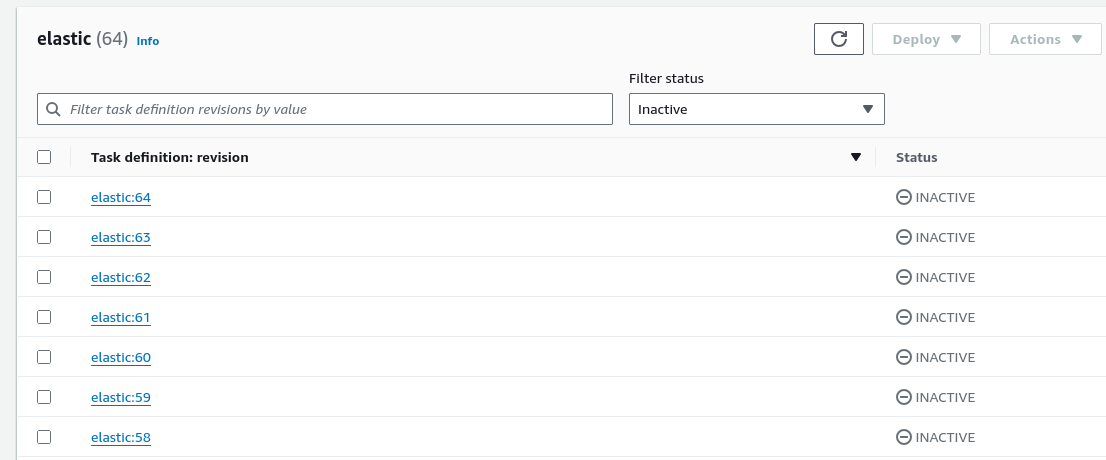
\includegraphics[width=\textwidth]{impl/definitions.png}
	\caption{Ejemplo de definciones de tareas de ECS en AWS}
	\label{fig:definitions}
\end{figure}

\begin{figure}[H]
	\centering
	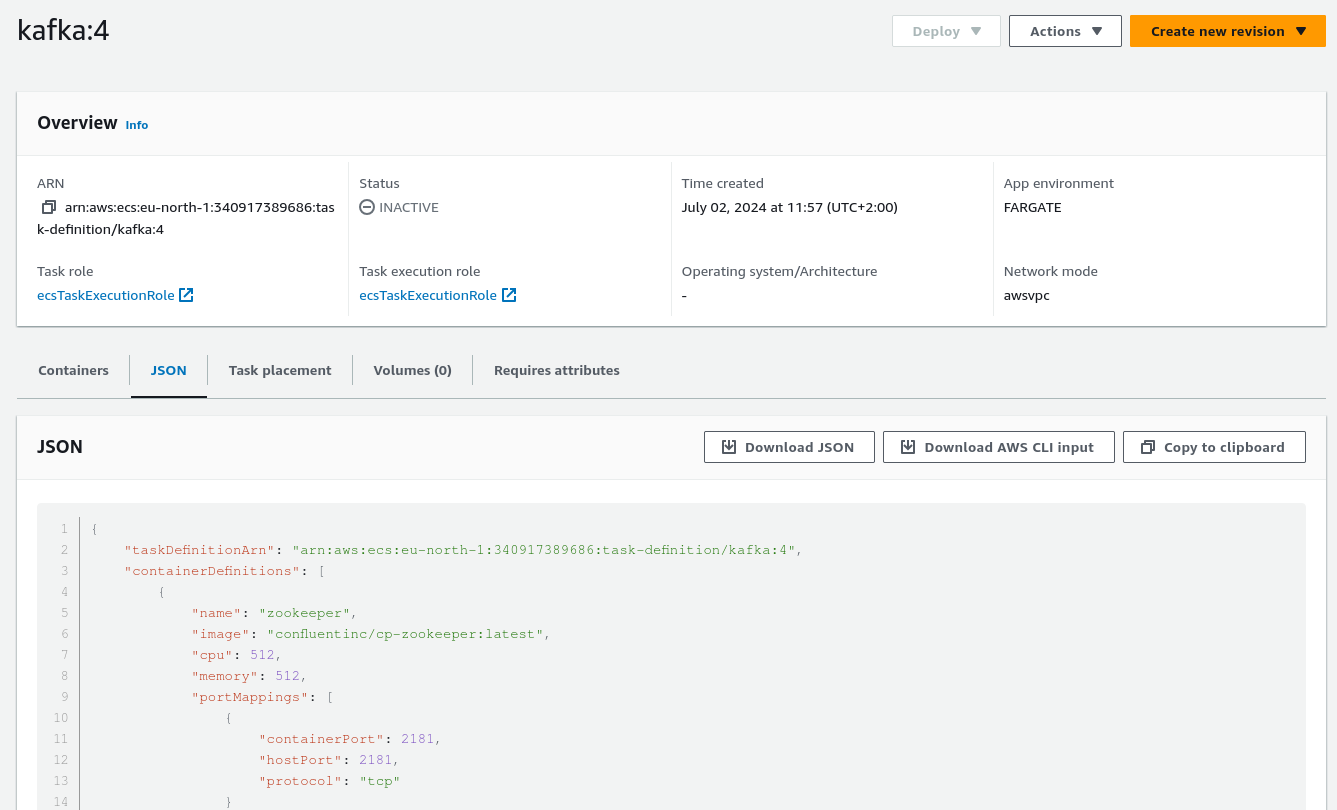
\includegraphics[width=\textwidth]{impl/ejemplo_definition.png}
	\caption{Ejemplo de definción de tarea (Kafka)}
	\label{fig:definition}
\end{figure}


\newpage{}
\subsection{Despliegue de la infraestructura}\label{subsec:impl_cloud_despliegue}
% TODO: desarrollar
% Aquí podría estar bien poner un diagrama de despliegue. Pero que se vea en el
% modelo que ese diagrama de despliegue no es el despliegue de tu proyecto.
% Es decir, el proyecto es crear un proceso de despliegue que hace un despliegue.
% Entonces que se vea que hay ese proceso y luego el diagrama de despliegue de lo
% que el proyecto permite desplegar


\newpage{}
\subsection{Explicación del código}\label{sec:impl_configuracion}
\emph{El código completo se encuentra en el anexo \fullref{anexo:cloud}.}

Los scripts de Terraform se dividen en varios archivos, cada uno de ellos con
una función específica, con el objetivo de facilitar la gestión y configuración
de los recursos y servicios. A continuación, se detallan dichos archivos y su
función en el proyecto.


\subsubsection{Recursos generales}


\subsubsection{Servicios de ELK}
